\chapter{Black Holes: From Something to Nothing}
\label{chap:black-holes}

Let us test the consequences of treating a simulated system and its simulator as two perspectives of the same underlying information.
Under this framework, a computer running a simulation and the simulated universe itself are simply dual descriptions of a single informational structure.

If this equivalence holds, what insight does it offer into the most bizarre and pathological object in our universe—one that classical physics still fails to fully comprehend? 

The black hole singularity.

According to General Relativity, all matter crossing the event horizon eventually collapses into a point of zero spatial volume and infinite density.
An entire star—millions or even billions of times more massive than the Earth is compressed into a region of vanishing volume.

By constructing a black hole simulation and treating the program execution and the emergent spacetime geometry as equivalent informational states, 
we can perpahs gain an entirely new perspective on these pathological points in classical geometry.



\section*{The Simulation of Gravitational Collapse}

Let us consider a black hole simulation tracking a massive, spherical dust cloud as it collapses under its own gravity to form a singularity.
In computational practice, we cannot run such a simulation to its absolute mathematical conclusion.
As the collapse approaches its final state, the software inevitably crashes.

This failure is driven by two factors: the fundamental breakdown of the classical Einstein field equations and the inherent limitations of floating-point precision.
Long before the physical singularity is reached, the execution trace is overwhelmed by division-by-zero exceptions and numerical infinities that instantly exceed the bit-width 
precision of the system's hardware. 



\subsection*{The Execution Trace as Spacetime}

Computers are deterministic state machines.
Each executed CPU instruction drives the system from one discrete state to the next.
In software engineering, an \textbf{execution trace} is the chronological record of this state trajectory.

Falling particles has many attribues, such as temperature. However, because General Relativity is fundamentally a theory of geometry, 
the ultimate nature of this computational breakdown must be geometric. So in this simulation, we will focus on the geometric configuration of the dust cloud and its spacetime fabric.

We therefore map each falling particle and every discrete coordinate of the spacetime fabric to a unique sequence of memory bits.
The execution trace of the simulation is then equivalent to a continuous bitstring representing successive temporal slices of the spatial configuration 
of the dust cloud.

Whatever happens in the simulation, must emergre from the information encoded in the bitstring, the execution trace.

And there are not too many attributes in bitstrings. A bitstring is a sequence of zeros and ones. It is a discrete, finite object. It's only attribute are its 
length, which is fixed in this case, and entropy. Entropy describes its \emph{informational content}, the amount of information it encodes.


\subsection{The Singularity as a State of Zero Informational Entropy}

Initially, the bitstring encoding the highly disordered dust cloud possesses maximum entropy and high descriptive complexity:

\begin{verbatim}
00100101011110101010101001010100101010101010101001001001110101010010100101010...
...
\end{verbatim}

As the simulation evolves toward a black hole, the \emph{entropy}  of the bitstring encoding the spatial geometry decreases.


\begin{verbatim}
...
0001000010000010010001000000001000100000000000001000010000000010000000100010000...
0001001000000000010000000000000010000010000000001000000000000000000100000000001...
0000001000000000000000000000001000000000000000000000100001000000000000000000100...
...
[hardware exception: division by zero / arithmetic overflow]
\end{verbatim}

Even though numerical instabilities prevent the machine to run the simulation to its completion, the entropy trend is clear.
By extrapolating the trend of the entropy of the execution trace, we arrive at a definitive conclusion: The black hole singularity corresponds to a state of zero informational entropy.

\begin{figure}[h!]
\centering
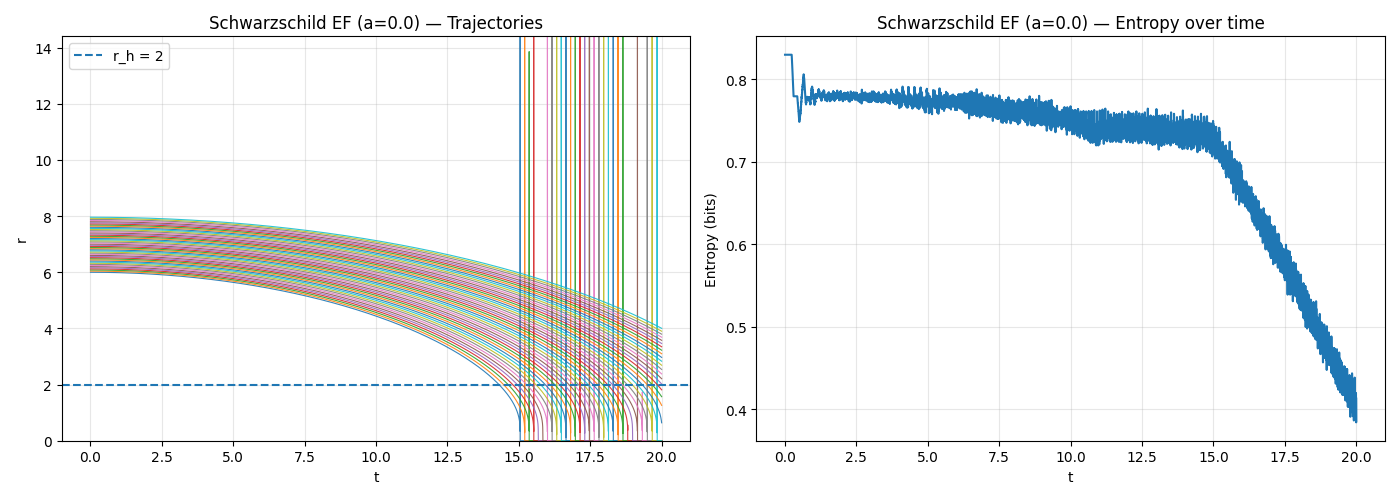
\includegraphics[width=1.0\textwidth]{figures/schwarzschild.png}
\caption{Execution-trace entropy of particles falling into a Schwarzschild black hole.}
\label{fig:schwarzschild-entropy}
\end{figure}


\section{Conclusion: The Exhaustion of Information}

In classical physics, gravitational curvature diverges to infinity because physical geodesics converge to a point with infinite density and curvature. 
However, our informational approach suggests that this infinity is merely a artifact of an exhausted descriptive framework. 
It is analogous to the mathematical divergence of surface derivatives when evaluating coordinates at the exact North Pole of a smooth sphere.

Remarkably, this zero-entropy conclusion is entirely invariant under coordinate choice, representational mapping, or dimensionality.
If you map a zero-entropy bitstring (such as a string consisting entirely of zeros) back to a geometric interpretation, it can only yield one possible object:
a single, featureless point.

Thus, singularities might not be terrifying regions of infinite physical massiveness, but the exact opposite: states of complete informational exhaustion.
They are the simplest, most trivial geometric configurations possible.

Because a zero-entropy bitstring is fundamentally incapable of encoding or describing internal microstructures, such as the discrete states of incoming particles, 
it offers a solution to the paradox of the singularity:

The probability of any falling particle actually reaching the singularity is zero. The singularity is simply too trivial to describethem.

And if the singularity cannot encode any information about the particles that fell into it, then it cannot contribute stress energy tensor of General Relativity.

Unlike the classical picture of a singularity as a region of infinite density, our informational perspective suggests that the singularity is actually a region of zero density. 
The geometry of the singularity is smooth. 


